% Course report, 10-page version: a short paper with only the main question, what was built, what was found and what it
% means (the full version is report.tex, the 20-page one report_short.tex). Numbers of the main comparison come from the
% macros and tables python -m ecgaug.paper writes into generated/; the few typed by hand are copied from report/results.md
% and checked against it. Build: cd report && tectonic report_brief.tex (figures come from ../figures/).
\documentclass[11pt]{article}
\usepackage[margin=2.5cm]{geometry}
\usepackage{microtype}
\usepackage{booktabs}
\usepackage{graphicx}
\usepackage{adjustbox}
\usepackage{amsmath}
\usepackage{xcolor}
\usepackage{hyperref}
\hypersetup{hidelinks}
\graphicspath{{../figures/}}
\usepackage{placeins}  % \FloatBarrier only where a figure must stay in its section
\renewcommand{\topfraction}{0.9}\renewcommand{\bottomfraction}{0.8}\renewcommand{\textfraction}{0.07}
\renewcommand{\floatpagefraction}{0.75}\setcounter{topnumber}{3}\setcounter{totalnumber}{5}
\newcommand{\missing}[1]{\textcolor{red}{[#1]}}
% Generated by python -m ecgaug.paper; do not edit. Every value comes from a result file.
\newcommand{\CountTestF}{388}
\newcommand{\CountTestN}{44,259}
\newcommand{\CountTestS}{1,837}
\newcommand{\CountTestV}{3,221}
\newcommand{\CountTrainingF}{388}
\newcommand{\CountTrainingN}{35,496}
\newcommand{\CountTrainingS}{644}
\newcommand{\CountTrainingV}{3,030}
\newcommand{\CountValidationF}{27}
\newcommand{\CountValidationN}{10,370}
\newcommand{\CountValidationS}{300}
\newcommand{\CountValidationV}{758}
\newcommand{\PhaseOneInputRepresentationAMean}{0.164}
\newcommand{\PhaseOneInputRepresentationBMean}{0.001}
\newcommand{\PhaseOneInputRepresentationCMean}{0.296}
\newcommand{\PhaseOneInputRepresentationDMean}{0.035}
\newcommand{\PhaseTwoBaselineClassifiersAMean}{0.349}
\newcommand{\PhaseTwoBaselineClassifiersBMean}{0.231}
\newcommand{\PhaseTwoBaselineClassifiersCMean}{0.315}
\newcommand{\PhaseTwoBaselineClassifiersDMean}{0.252}
\newcommand{\PhaseOneWinner}{C}
% Written by ecgaug.final_eval; do not edit.
\newcommand{\TestCnnNoneRare}{0.088}
\newcommand{\TestCnnNoneRareLow}{0.037}
\newcommand{\TestCnnNoneRareHigh}{0.194}
\newcommand{\TestCnnClassWeightedRare}{0.113}
\newcommand{\TestCnnClassWeightedRareLow}{0.057}
\newcommand{\TestCnnClassWeightedRareHigh}{0.207}
\newcommand{\TestCnnRandomOversamplingRare}{0.136}
\newcommand{\TestCnnRandomOversamplingRareLow}{0.061}
\newcommand{\TestCnnRandomOversamplingRareHigh}{0.247}
\newcommand{\TestCnnSmoteRare}{0.070}
\newcommand{\TestCnnSmoteRareLow}{0.025}
\newcommand{\TestCnnSmoteRareHigh}{0.172}
\newcommand{\TestCnnCvaeRare}{0.113}
\newcommand{\TestCnnCvaeRareLow}{0.049}
\newcommand{\TestCnnCvaeRareHigh}{0.217}
\newcommand{\TestCnnWganGpRare}{0.079}
\newcommand{\TestCnnWganGpRareLow}{0.033}
\newcommand{\TestCnnWganGpRareHigh}{0.164}
\newcommand{\TestRnnNoneRare}{0.075}
\newcommand{\TestRnnNoneRareLow}{0.014}
\newcommand{\TestRnnNoneRareHigh}{0.232}
\newcommand{\TestRnnClassWeightedRare}{0.061}
\newcommand{\TestRnnClassWeightedRareLow}{0.022}
\newcommand{\TestRnnClassWeightedRareHigh}{0.168}
\newcommand{\TestRnnRandomOversamplingRare}{0.090}
\newcommand{\TestRnnRandomOversamplingRareLow}{0.028}
\newcommand{\TestRnnRandomOversamplingRareHigh}{0.196}
\newcommand{\TestRnnSmoteRare}{0.086}
\newcommand{\TestRnnSmoteRareLow}{0.025}
\newcommand{\TestRnnSmoteRareHigh}{0.206}
\newcommand{\TestRnnCvaeRare}{0.073}
\newcommand{\TestRnnCvaeRareLow}{0.035}
\newcommand{\TestRnnCvaeRareHigh}{0.157}
\newcommand{\TestRnnWganGpRare}{0.069}
\newcommand{\TestRnnWganGpRareLow}{0.027}
\newcommand{\TestRnnWganGpRareHigh}{0.156}
\newcommand{\TestCnnCvaeVsNoneDiff}{0.025}
\newcommand{\TestCnnCvaeVsNoneLow}{-0.018}
\newcommand{\TestCnnCvaeVsNoneHigh}{0.047}
\newcommand{\TestCnnCvaeVsNonePHolm}{1.0000}
\newcommand{\TestCnnWganGpVsNoneDiff}{-0.009}
\newcommand{\TestCnnWganGpVsNoneLow}{-0.045}
\newcommand{\TestCnnWganGpVsNoneHigh}{0.015}
\newcommand{\TestCnnWganGpVsNonePHolm}{1.0000}
\newcommand{\TestRnnCvaeVsNoneDiff}{-0.002}
\newcommand{\TestRnnCvaeVsNoneLow}{-0.100}
\newcommand{\TestRnnCvaeVsNoneHigh}{0.032}
\newcommand{\TestRnnCvaeVsNonePHolm}{1.0000}
\newcommand{\TestRnnWganGpVsNoneDiff}{-0.006}
\newcommand{\TestRnnWganGpVsNoneLow}{-0.138}
\newcommand{\TestRnnWganGpVsNoneHigh}{0.035}
\newcommand{\TestRnnWganGpVsNonePHolm}{1.0000}
\newcommand{\TestCnnCvaeVsWganGpDiff}{0.034}
\newcommand{\TestCnnCvaeVsWganGpLow}{-0.002}
\newcommand{\TestCnnCvaeVsWganGpHigh}{0.068}
\newcommand{\TestCnnCvaeVsWganGpPHolm}{0.5504}
\newcommand{\TestCnnCvaeVsSmoteDiff}{0.044}
\newcommand{\TestCnnCvaeVsSmoteLow}{-0.029}
\newcommand{\TestCnnCvaeVsSmoteHigh}{0.072}
\newcommand{\TestCnnCvaeVsSmotePHolm}{1.0000}
\newcommand{\TestCnnCvaeVsClassWeightedDiff}{0.001}
\newcommand{\TestCnnCvaeVsClassWeightedLow}{-0.041}
\newcommand{\TestCnnCvaeVsClassWeightedHigh}{0.042}
\newcommand{\TestCnnCvaeVsClassWeightedPHolm}{1.0000}
\newcommand{\TestCnnCvaeVsRandomOversamplingDiff}{-0.022}
\newcommand{\TestCnnCvaeVsRandomOversamplingLow}{-0.074}
\newcommand{\TestCnnCvaeVsRandomOversamplingHigh}{0.010}
\newcommand{\TestCnnCvaeVsRandomOversamplingPHolm}{1.0000}
\newcommand{\TestRnnCvaeVsWganGpDiff}{0.004}
\newcommand{\TestRnnCvaeVsWganGpLow}{-0.027}
\newcommand{\TestRnnCvaeVsWganGpHigh}{0.065}
\newcommand{\TestRnnCvaeVsWganGpPHolm}{1.0000}
\newcommand{\TestRnnCvaeVsSmoteDiff}{-0.013}
\newcommand{\TestRnnCvaeVsSmoteLow}{-0.067}
\newcommand{\TestRnnCvaeVsSmoteHigh}{0.016}
\newcommand{\TestRnnCvaeVsSmotePHolm}{1.0000}
\newcommand{\TestRnnCvaeVsClassWeightedDiff}{0.012}
\newcommand{\TestRnnCvaeVsClassWeightedLow}{-0.047}
\newcommand{\TestRnnCvaeVsClassWeightedHigh}{0.039}
\newcommand{\TestRnnCvaeVsClassWeightedPHolm}{1.0000}
\newcommand{\TestRnnCvaeVsRandomOversamplingDiff}{-0.016}
\newcommand{\TestRnnCvaeVsRandomOversamplingLow}{-0.059}
\newcommand{\TestRnnCvaeVsRandomOversamplingHigh}{0.016}
\newcommand{\TestRnnCvaeVsRandomOversamplingPHolm}{1.0000}



\title{Same Model, New Patient:\\ Can Synthetic Heartbeats Rescue Rare-Arrhythmia Detection?\\[6pt]
\large Rare-Arrhythmia Detection with Generative ECG Augmentation\\[2pt]\normalsize Course project, short paper}
\author{\begin{tabular}{c@{\hspace{3em}}c}Akash Saha (261110401) & Kartheek Dasari (261110029)\\
 H M Karthik (261110025) & T D Manindra (261050084)\end{tabular}}
\date{}

\begin{document}
\maketitle

\begin{abstract}
\noindent Tested on beats of the patients it was trained on, our heartbeat classifier detects the rare arrhythmia classes with a
rare-class F1 of 0.837. Tested on patients it has never seen, it scores \TestCnnNoneRare. We asked whether class-conditional
generative models, a conditional VAE and a WGAN-GP, can close that gap by synthesising the rare beats that are missing. Under rules
registered before any test record was read, with training and test patients strictly apart, we compared both generators with no
augmentation, a class-weighted loss, random oversampling and SMOTE for two classifiers, and read the 22 test patients once.
Generative augmentation did not detectably help: the best case, the CNN with the cVAE, gained $+\TestCnnCvaeVsNoneDiff$ (95\% CI
$\TestCnnCvaeVsNoneLow$ to $+\TestCnnCvaeVsNoneHigh$). Twenty-three pre-registered follow-up analyses then found what does help:
describing each beat relative to the patient's own beats, judging prematurity against the patient's own rhythm, vetoing S calls during
atrial fibrillation and averaging ten runs raised the test score to 0.587, level with the best published inter-patient result. Every
prediction comes with a saliency map and a note whose every claim is checked against the model's output.
\end{abstract}

\section{Introduction}
A heartbeat classifier can look excellent or useless on the same data. Trained on the MIT-BIH Arrhythmia Database~\cite{moody2001}
with its beats split at random, our convolutional network finds the rare arrhythmia beats with a rare-class F1 of 0.837. Trained on
one group of patients and tested on another, the same network scores \TestCnnNoneRare. Nothing about the network changed; only the
patients did (Figure~\ref{fig:gap}).

\begin{figure}[htbp]\centering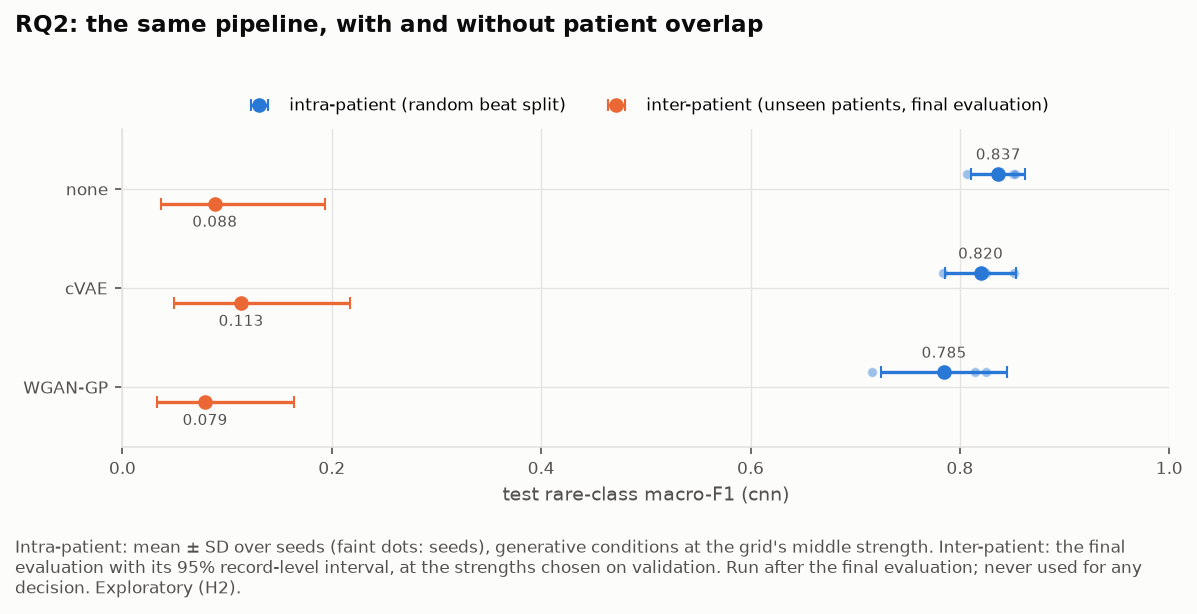
\includegraphics[width=0.92\linewidth]{phase4_leakage_audit/intra_vs_inter.png}
\caption{The same pipeline, scored on held-out beats of the training patients (blue) and on patients it has never seen (orange).
The rare-class macro-F1 falls from about 0.8 to about 0.1, with or without generative augmentation.}\label{fig:gap}\end{figure}

The reason is that patients differ. A heartbeat's shape depends on the heart, the electrode position and the disease, and the beats
that matter most are both rare and concentrated in a few people: supraventricular ectopic beats (S), whose burden goes with later
atrial fibrillation and stroke~\cite{binici2010}, and fusion beats (F). A model that has seen a few hundred S beats from a dozen people
has to recognise them in someone new.

Generative models offer an apparent way out: learn what the rare beats look like and manufacture more of them. Conditional
VAEs~\cite{sohn2015cvae} and Wasserstein GANs~\cite{gulrajani2017wgangp} can draw convincing synthetic ECG, and augmenting with them is
often reported to help, mostly on splits where the test patients were also in training. We asked the question a clinic would ask:
\begin{quote}\itshape
With training and test patients strictly apart, does class-conditional generative augmentation improve detection of the rare classes
S and F, compared with no augmentation, a class-weighted loss, random oversampling and SMOTE?
\end{quote}
We built the whole pipeline (data, two classifiers, two generator families, augmentation, saliency maps and fact-checked notes) and
ran it in phases. Each phase ended with a gate at which a rule registered in advance chose on validation patients only, and the test
patients were read once, at the end; 761 runs are logged. This paper reports four findings:
\begin{itemize}\setlength{\itemsep}{1pt}
\item \textbf{The pre-registered answer is no.} Generative augmentation did not detectably improve rare-class detection on new
patients; it performed on par with the cheap balancing methods (Section~\ref{sec:answer}).
\item \textbf{Patient overlap inflates the score almost tenfold}, so scores from random beat splits say little about new patients
(Section~\ref{sec:gap}).
\item \textbf{Realistic synthetic beats are not useful beats}: no synthetic-quality metric predicted the gain (Section~\ref{sec:quality}).
\item \textbf{What does help is knowing the patient}: 23 follow-up analyses, each registered before it ran, raised the test score from
\TestCnnCvaeRare\ to 0.587 and tested it on 977 patients no analysis had used (Section~\ref{sec:followup}).
\end{itemize}

\section{Data and rules}\label{sec:data}
\paragraph{Data.} The MIT-BIH Arrhythmia Database~\cite{moody2001,goldberger2000} holds 48 half-hour two-lead recordings whose beats
were labelled by cardiologists. We use lead MLII at 360~Hz, map the labels to the AAMI classes~\cite{aami2012ec57} N (normal),
S (supraventricular ectopic), V (ventricular ectopic) and F (fusion), and leave out the four paced records. Figure~\ref{fig:beats}
shows what the classes look like.

\begin{figure}[htbp]\centering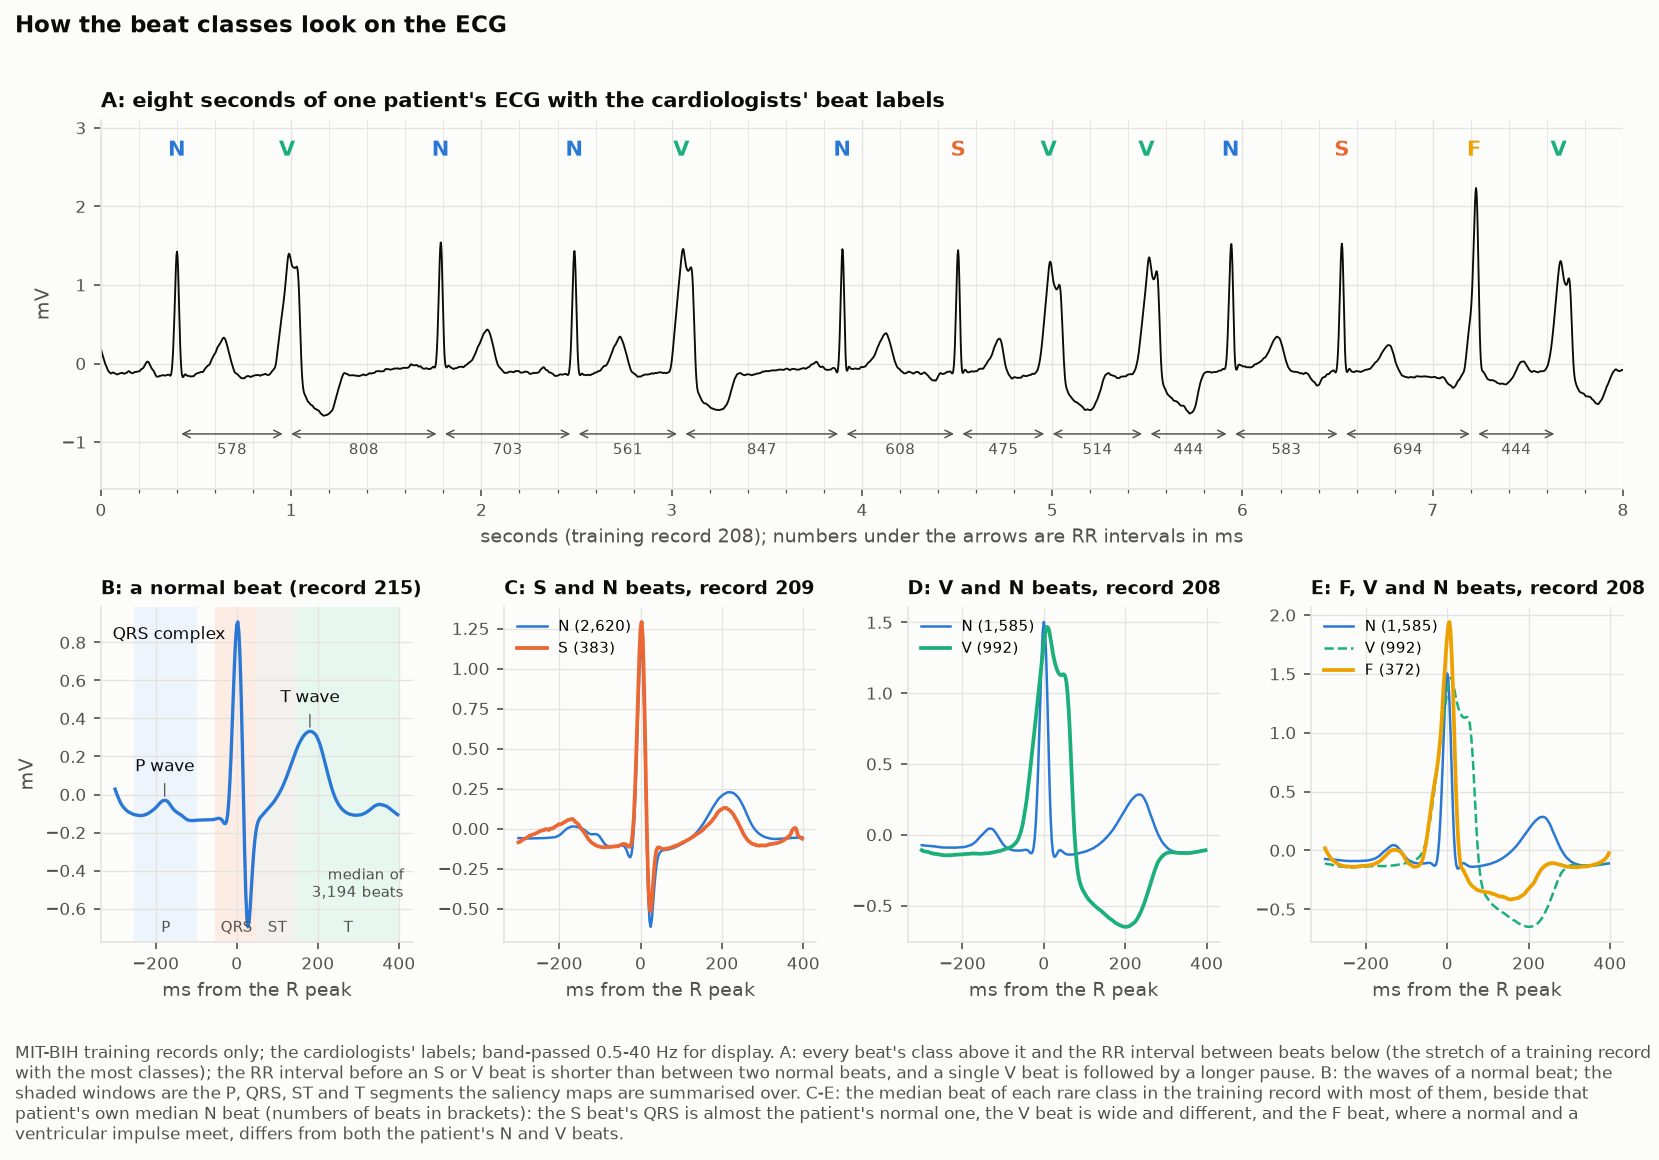
\includegraphics[width=0.95\linewidth]{report/medical_background.png}
\caption{The beat classes on the ECG (training records only). An S beat comes early but looks almost like the patient's normal beat;
a V beat is wide and different; an F beat lies between the two. The RR intervals (arrows) are what reveals an early beat.}
\label{fig:beats}\end{figure}

\paragraph{Patients kept apart.} We use the split of de Chazal et al.~\cite{dechazal2004}: 22 records (DS1) for training and
validation, the other 22 (DS2) for the test, so no patient is in two splits; five DS1 patients form the validation set
(Table~\ref{tab:data}). Generators, oversamplers and normalisation see training patients only.

\begin{table}[htbp]\centering\small% Generated by python -m ecgaug.paper from: results/phase1_data/record_counts.csv
\begin{tabular}{lrrrrr}
\toprule
Split & Records & N & S & V & F \\
\midrule
training & 17 & 35,496 & 644 & 3,030 & 388 \\
validation & 5 & 10,370 & 300 & 758 & 27 \\
test (DS2) & 22 & 44,259 & 1,837 & 3,221 & 388 \\
\bottomrule
\end{tabular}

\caption{Records and beats per split. S beats are under 4\% of each split, and F beats at most 1\%.}\label{tab:data}\end{table}

\paragraph{Measure and rules.} The primary measure is the rare-class macro-F1, the mean F1 of S and F on the test patients, with
95\% confidence intervals from a bootstrap over patients and Holm's correction~\cite{holm1979} for the four confirmatory comparisons.
Every selection rule and hypothesis was registered before the experiment it governs, and each phase ended with a gate at which the
rule was applied and approved. The test file opens only for the final evaluation, and every read is logged. The follow-up analyses
were registered as new versions of the rules (21 in all) before they ran, and are reported apart from the primary results.

\section{The system}\label{sec:system}
Figure~\ref{fig:flow} shows the pipeline. Each stage was chosen on validation patients:
\begin{itemize}\setlength{\itemsep}{1pt}
\item \textbf{Beat:} a 0.5~s window around the R peak, z-scored, with the RR intervals before and after the beat as extra input
(the best of four representations).
\item \textbf{Classifiers:} a shallow CNN (73k parameters) and a BiLSTM (135k), the best of four architectures; pretraining on
PTB-XL did not help.
\item \textbf{Generators:} a conditional VAE and a WGAN-GP, each the best of four designs, trained with three seeds into frozen
banks of synthetic beats.
\item \textbf{Augmentation:} each rare class brought up to a fraction (0.1, 0.25 or 0.5) of the N count with synthetic beats, keeping
those closest to real training beats by dynamic time warping; the fraction chosen per condition. With no augmentation, the
class-weighted loss, random oversampling and SMOTE~\cite{chawla2002smote} this made a 96-run grid.
\item \textbf{Explanation and note:} Grad-CAM~\cite{selvaraju2016gradcam} for the CNN and occlusion for the BiLSTM, summarised as the
share of attention in the P, QRS, ST and T windows; a language model (Gemini) writes a note from a JSON of the model's output only,
and a fact checker rejects any number, class or finding not in that JSON.
\end{itemize}

\begin{figure}[htbp]\centering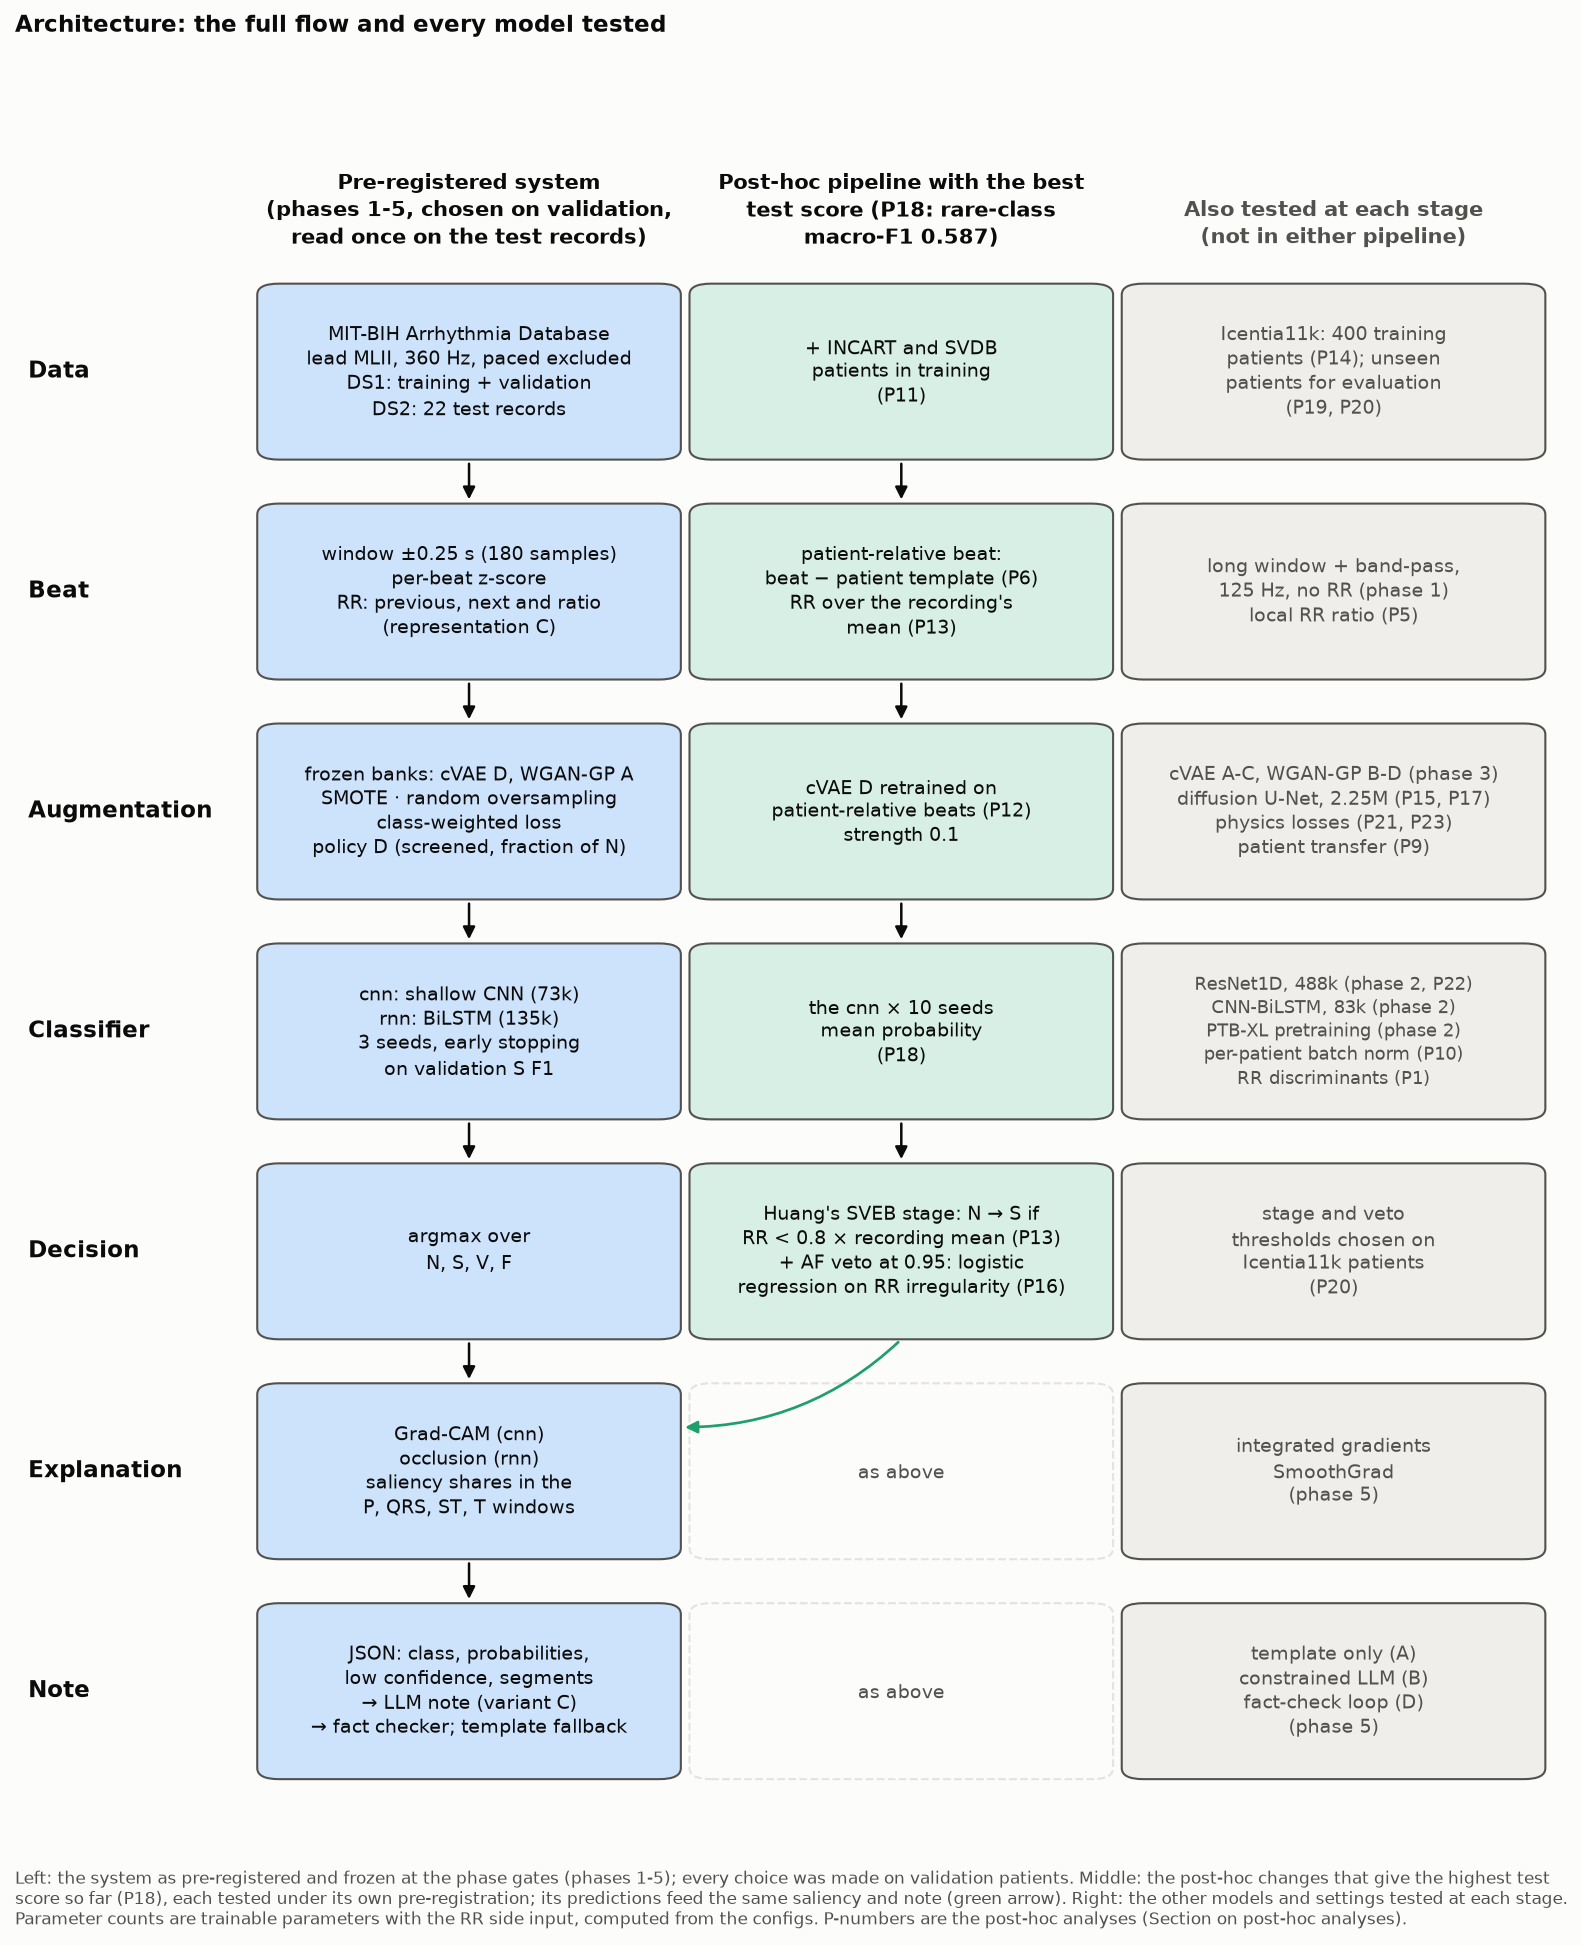
\includegraphics[width=0.8\linewidth]{architecture/flow.png}
\caption{The pipeline. Left: the pre-registered system. Middle: the follow-up pipeline with the best test score (Section~\ref{sec:followup}).
Right: what else was tested at each stage.}\label{fig:flow}\end{figure}

\section{Results}\label{sec:results}
Four hypotheses were registered before any test record was read (Table~\ref{tab:hypotheses}); the verdicts are the registered rules
applied as written. The sections below give the evidence behind each.

\begin{table}[htbp]\centering\small\adjustbox{max width=\linewidth}{% Generated by python -m ecgaug.paper from the result files
\begin{tabular}{lp{5.2cm}lp{5.2cm}}
\toprule
Hypothesis & Statement & Verdict & Evidence \\
\midrule
H1 & confirmatory: a generative condition improves test rare-class macro-F1 over none (Holm, 4 tests) & not supported & no confirmatory comparison significant \\
H1b & exploratory: gains larger for F than for S & mixed & F gain larger than S gain in 2 of 4 generative conditions \\
H1c & secondary: generative beats SMOTE, random oversampling and class-weighted loss & not supported & 0 of 6 comparisons of the best generative condition with a baseline significant \\
H2 & exploratory: intra-patient evaluation inflates the baseline and the gains & not consistent & inflation of the baseline +0.748; larger intra-patient gain for 0 of 2 generators \\
H3 & exploratory: a quality metric predicts the downstream gain & not supported & 0 of 5 metrics with an interval excluding zero \\
H4 & exploratory: augmented models are at least as faithful as the baseline & mixed & augmented faithfulness at least the baseline's in 1 of 4 model pairs \\
\bottomrule
\end{tabular}
}
\caption{The pre-registered hypotheses, their verdicts and the evidence, all on the 22 test patients.}\label{tab:hypotheses}\end{table}

\subsection{The pre-registered answer}\label{sec:answer}
Table~\ref{tab:test} gives the single test read. For the CNN, training without augmentation scored \TestCnnNoneRare, the cVAE
\TestCnnCvaeRare\ and the WGAN-GP \TestCnnWganGpRare, against \TestCnnClassWeightedRare\ for the class-weighted loss and
\TestCnnRandomOversamplingRare\ for random oversampling. The cVAE's gain over no augmentation, $+\TestCnnCvaeVsNoneDiff$ (95\% CI
$\TestCnnCvaeVsNoneLow$ to $+\TestCnnCvaeVsNoneHigh$), points the right way, and it nearly tripled the CNN's sensitivity for F beats, from
0.064 to 0.185. But no confirmatory comparison survived Holm's correction, and the cVAE was level with the cheap methods
($+\TestCnnCvaeVsClassWeightedDiff$ against the class-weighted loss, $\TestCnnCvaeVsRandomOversamplingDiff$ against random
oversampling). For the BiLSTM the differences were smaller still. The hypothesis is not supported at this sample size.

\begin{table}[htbp]\centering\small\begin{tabular}{llrrr}
\toprule
Architecture & Condition & Strength & Rare macro-F1 [95\% CI] & N recall \\
\midrule
cnn & none & -- & 0.088 [0.037, 0.194] & 0.962 \\
cnn & class weighted & 0.5 & 0.113 [0.057, 0.207] & 0.933 \\
cnn & random oversampling & 0.1 & 0.136 [0.061, 0.247] & 0.844 \\
cnn & smote & 0.1 & 0.070 [0.025, 0.172] & 0.985 \\
cnn & cvae & 0.25 & 0.113 [0.049, 0.217] & 0.938 \\
cnn & wgan gp & 0.1 & 0.079 [0.033, 0.164] & 0.955 \\
rnn & none & -- & 0.075 [0.014, 0.232] & 0.961 \\
rnn & class weighted & 0.75 & 0.061 [0.022, 0.168] & 0.865 \\
rnn & random oversampling & 0.1 & 0.090 [0.028, 0.196] & 0.883 \\
rnn & smote & 0.1 & 0.086 [0.025, 0.206] & 0.894 \\
rnn & cvae & 0.1 & 0.073 [0.035, 0.157] & 0.926 \\
rnn & wgan gp & 0.5 & 0.069 [0.027, 0.156] & 0.857 \\
\bottomrule
\end{tabular}

\caption{The 22 test patients, read once: rare-class macro-F1 with 95\% intervals from a bootstrap over patients, and the recall of
normal beats. The strength is the fraction of the N count chosen on validation.}\label{tab:test}\end{table}

\subsection{Patient overlap inflates the score}\label{sec:gap}
After the final evaluation, the same CNN was trained and tested on a random beat split of all 44 records. Without augmentation it
reached 0.837 $\pm$ 0.026 (Figure~\ref{fig:gap}), and 0.803 and 0.777 on two further random splits. The generators did not help
there either (cVAE $-0.017$, WGAN-GP $-0.052$). A model tested on the patients it was trained on is largely tested on its memory of
those patients: published results with random splits above 0.9~\cite{kwak2024diffusion} and inter-patient results around
0.5--0.6~\cite{huang2014,zhu2022} measure different things.

\subsection{Realistic synthetic beats are not useful beats}\label{sec:quality}
We first checked that the quality metrics rank deliberately degraded beats correctly (dynamic time warping and a spectral distance
did; a Fr\'echet-distance analogue and train-on-synthetic-test-on-real did not). Five metrics, covering fidelity, diversity,
memorization and a classifier two-sample test, were then compared with the downstream gain over 96 checkpoints of 24 generator
runs. None predicted it (Spearman $\rho$ from $-0.20$ to $+0.18$, every interval including zero). A follow-up analysis shows why:
57--65\% of the synthetic S beats lie nearest to a single training patient, record 209, just as 60\% of the real training S beats do,
while the validation patients' S beats lie nearest to training patients who contribute only 1--2\% of them. The generators
reproduce the training patients faithfully, and that is not what new patients need.

\subsection{What does help: knowing the patient}\label{sec:followup}
After the final evaluation, 23 follow-up analyses (P1--P23), each registered before it ran and reported apart, asked what does move
the score. Four changes mattered (Figure~\ref{fig:progress}):
\begin{enumerate}\setlength{\itemsep}{1pt}
\item \textbf{Each beat relative to the patient} (P7): subtracting the patient's own template beat raised the CNN without
augmentation from \TestCnnNoneRare\ to 0.371.
\item \textbf{Prematurity against the patient's rhythm} (P13): RR intervals divided by the recording's mean RR~\cite{lin2014}, and
Huang et al.'s rule that calls an early beat S~\cite{huang2014}, raised the cVAE condition to 0.523.
\item \textbf{No S calls during atrial fibrillation} (P16): a detector using RR intervals only, fitted on the MIT-BIH Atrial
Fibrillation Database~\cite{goldberger2000}, raised every condition by 0.018 to 0.034, each 95\% interval above zero.
\item \textbf{Ten runs averaged} (P18): the cVAE's ten-run ensemble reached 0.587 [0.086, 0.702], with S F1 0.647 and F F1 0.527.
\end{enumerate}

\begin{figure}[htbp]\centering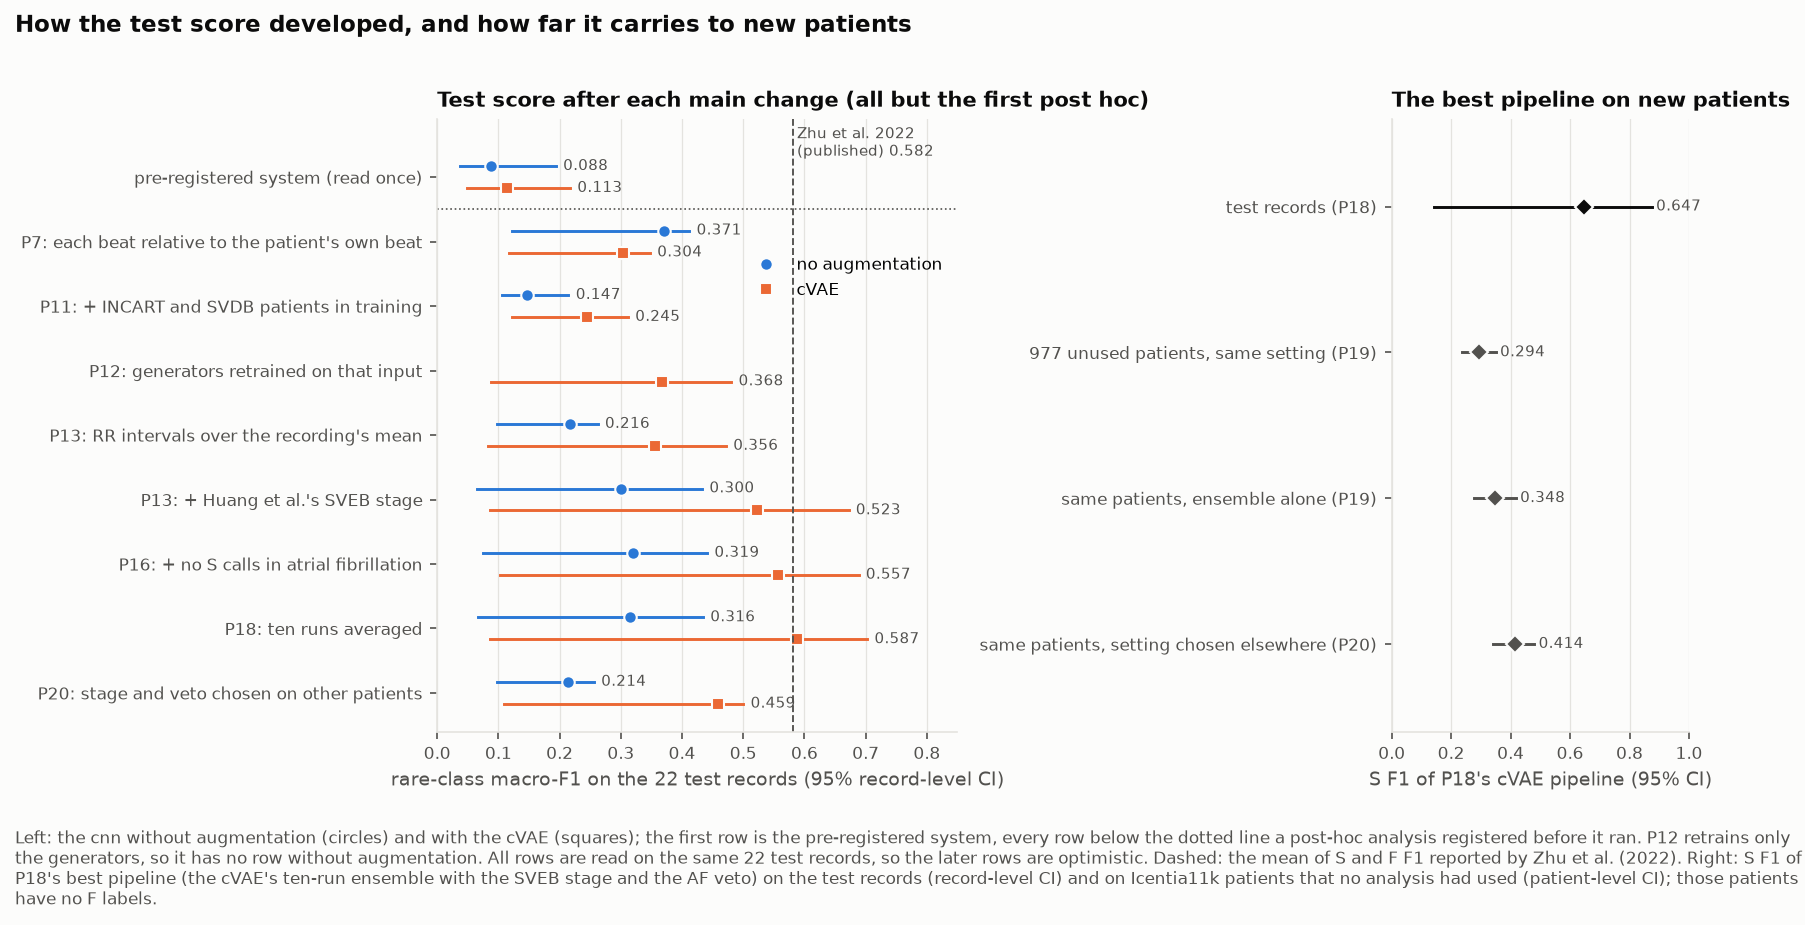
\includegraphics[width=\linewidth]{report/progress.png}
\caption{Left: the test score after each main change, without augmentation (circles) and with the cVAE (squares); every row below
the dotted line is a follow-up analysis. Right: the best pipeline's S F1 on the test patients and on unseen Icentia11k patients.}
\label{fig:progress}\end{figure}

\begin{table}[htbp]\centering\small
\begin{tabular}{lrrrr}\toprule
Inter-patient (DS2) results & S F1 & V F1 & F F1 & Mean of S and F F1 \\\midrule
de Chazal et al. 2004~\cite{dechazal2004} & 0.511 & 0.797 & -- & -- \\
Huang et al. 2014~\cite{huang2014} & 0.577 & 0.924 & -- & -- \\
Zhu et al. 2022~\cite{zhu2022} & \textbf{0.686} & \textbf{0.960} & 0.477 & 0.582 \\
Ours, pre-registered (CNN with the cVAE) & 0.173 & 0.893 & 0.054 & \TestCnnCvaeRare \\
Ours, follow-up P18 (cVAE ensemble, S stage, AF veto) & 0.647 & 0.936 & \textbf{0.527} & \textbf{0.587} \\\bottomrule
\end{tabular}
\caption{Beside published inter-patient results (F1 computed from the reported sensitivity and positive predictivity where a paper
gives no F1).}\label{tab:published}\end{table}

That places the best pipeline level with the best published inter-patient result (Table~\ref{tab:published}). It is also optimistic:
the follow-up analyses read the same 22 test patients many times. On 977 Icentia11k patients~\cite{tan2022icentia} that no analysis
had used, the same pipeline reached S F1 0.294 [0.237, 0.350], and 0.414 when its two thresholds were chosen on 388 other Icentia11k
patients; on the test records that choice gave 0.459, because one test record (232) holds 1,381 of the 1,836 usable test S beats and
no tuning patient resembles it. The cVAE gave the highest test score in P13, P16 and P18, but on the unseen patients it was level with
the other conditions (differences from $-0.001$ to $+0.008$, none detectable).

\subsection{A prediction a clinician can check}\label{sec:explain}
Of four saliency methods, the rule chose Grad-CAM for the CNN (the most faithful: deleting its most salient samples hurt the model
most) and occlusion for the BiLSTM. Of four note generators tried on 50 beats, all made zero unsupported claims; the rule chose
Gemini with worked examples and a fixed output schema, which covered every required fact in 2.6~s per note. The demo
(Figure~\ref{fig:demo}) shows the whole chain for one beat: the offline analysis by our models, then a review written by Gemini from
those results only, with every claim it makes checked against them.

\begin{figure}[htbp]\centering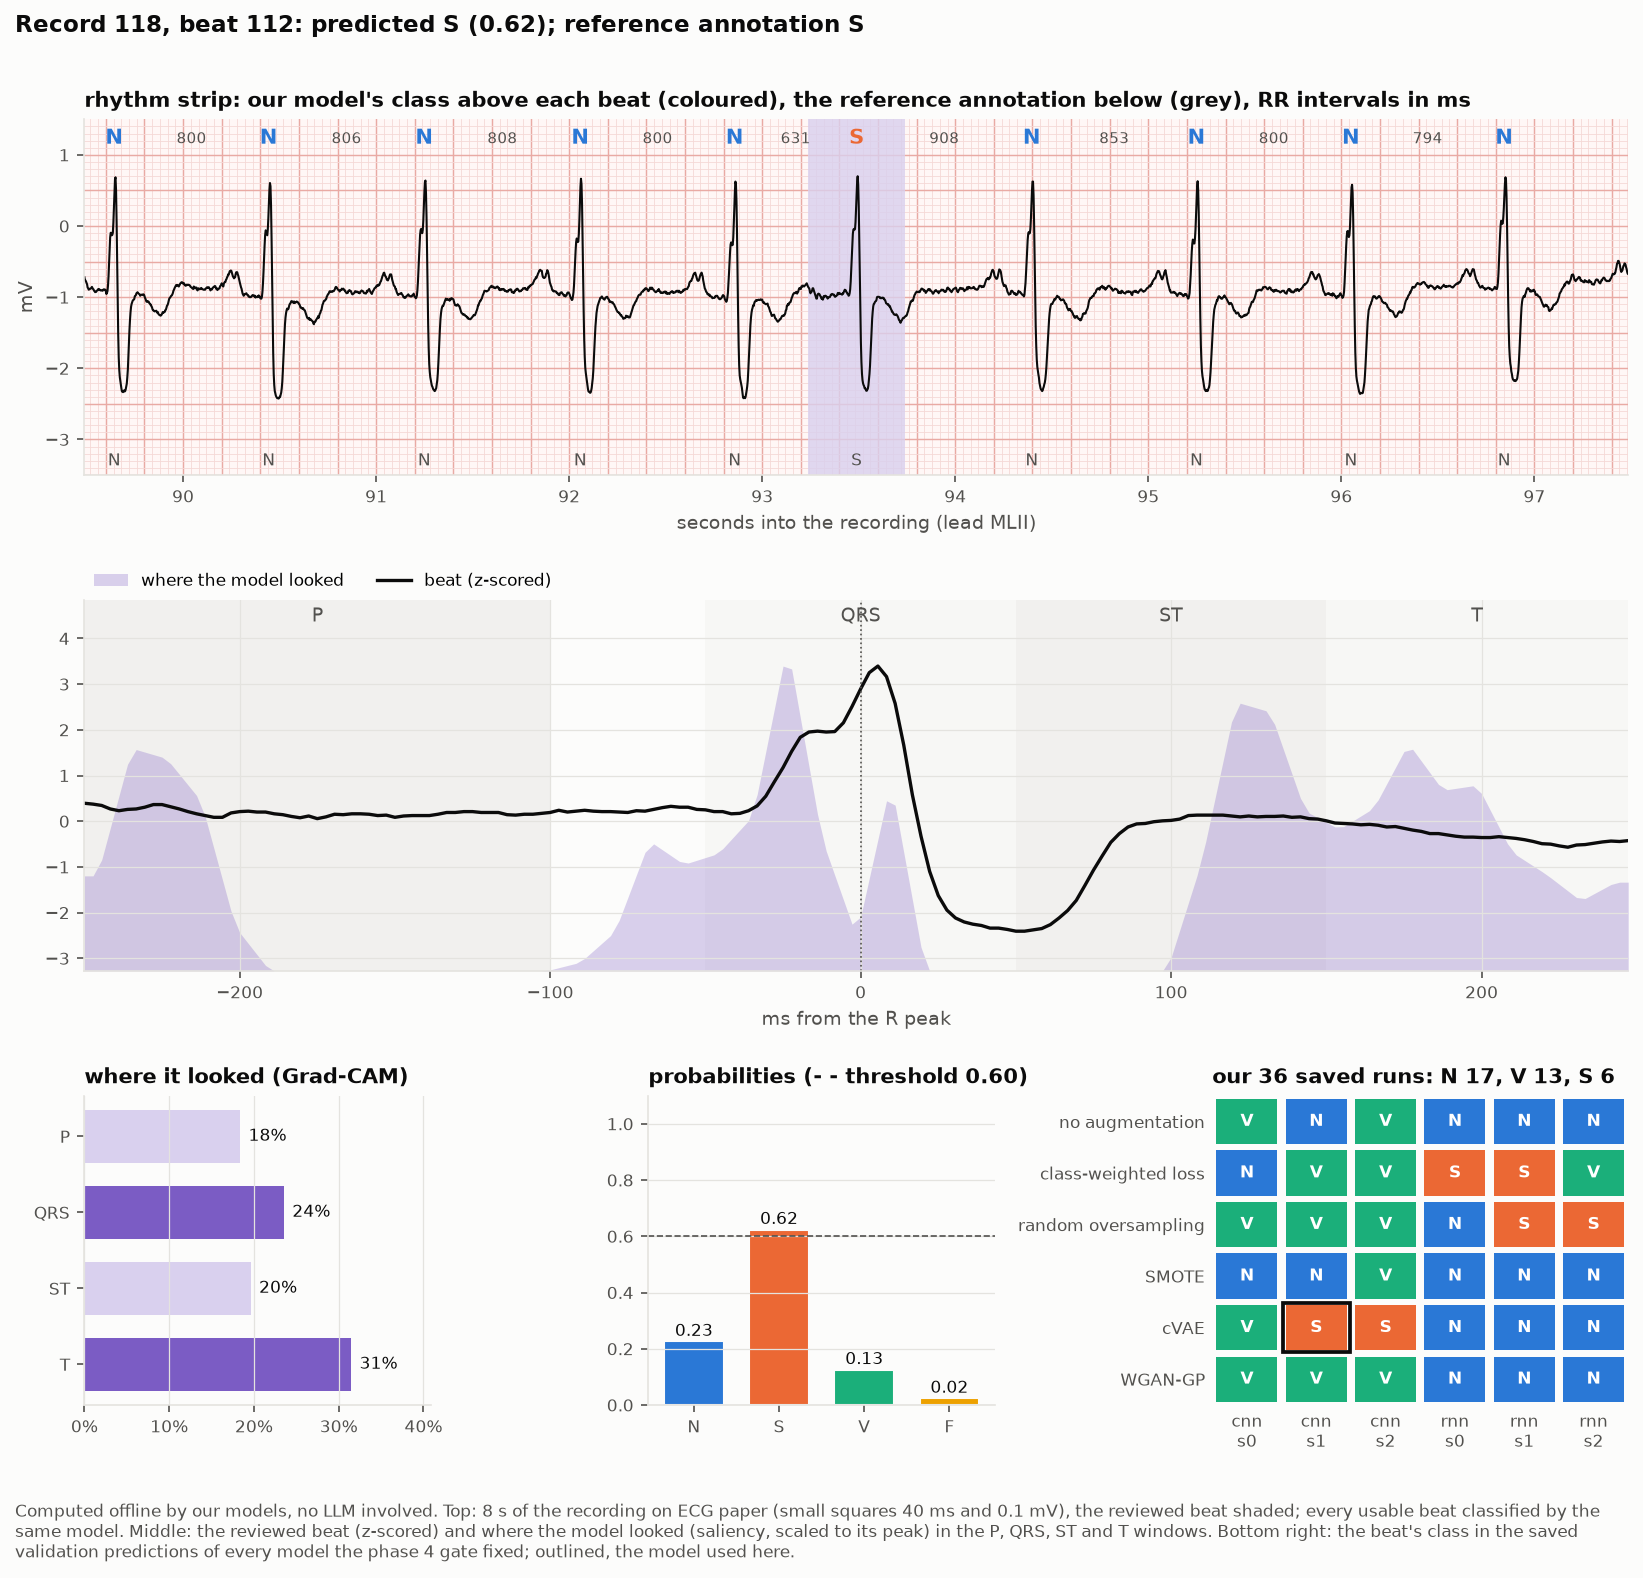
\includegraphics[width=0.72\linewidth]{demo_example/record118_beat112.png}
\caption{The demo for one S beat of a validation patient: the rhythm strip with each beat's predicted class and the reference label,
where the model looked, the probabilities, and how all 36 saved runs classified this beat (only 6 called it S).}
\label{fig:demo}\end{figure}

\FloatBarrier
\section{What it means}\label{sec:discussion}
\paragraph{Variety, not volume.} With 17 training patients, the bottleneck for new patients is not the number of rare beats but how
many different patients they come from. The generators multiplied the beats of the few patients they saw; what helped instead put
each beat in the context of its own patient, as a cardiologist reads a rhythm strip: is this beat early for this heart, does it differ
from this patient's normal beat, is the rhythm fibrillating?

\paragraph{The protocol decides the score.} The same network scores 0.837 or \TestCnnNoneRare\ depending only on whether the test
patients were seen in training. Results on random beat splits should not be compared with results on new patients.

\paragraph{Limitations.} The rare beats sit in very few patients (most test S beats in one record), so the intervals are wide;
records 201 and 202 come from the same person (the conclusions hold without record 202). The follow-up analyses are optimistic because
they read the same test patients; the unseen Icentia11k patients give the fairer estimate. The notes restate the model; they do not
diagnose.

\paragraph{Conclusion.} Under a strict inter-patient protocol, synthetic heartbeats from a cVAE or a WGAN-GP did not detectably improve
rare-arrhythmia detection over simple balancing. Patient-relative inputs, rhythm context and ensembles did, reaching the level of the
best published inter-patient result. Showing whether generative augmentation adds to that needs what it cannot manufacture: more
patients with rare beats.

\begingroup\footnotesize
\bibliographystyle{plain}
\bibliography{refs}
\endgroup
\end{document}
